\documentclass[../main.tex]{subfiles}
\graphicspath{{\subfix{../images/}}}


\begin{document}

\section{Overview of machine learning concepts}
\label{sec:ml_intro}

\begin{figure}[ht]
     \centering
     \begin{subfigure}[h]{0.40\textwidth}
         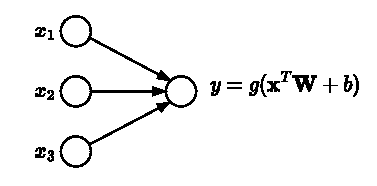
\includegraphics[width=\textwidth]{images/neural_network_node.drawio.pdf}
         \caption{}
         \centering
     \end{subfigure}
     \hfill
     \begin{subfigure}[h]{0.5\textwidth}
         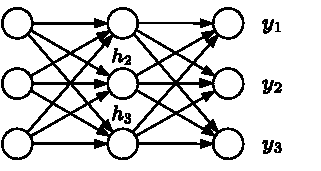
\includegraphics[width=\textwidth]{images/single_layer_nn.drawio.pdf}
         \caption{}
        \centering
    \end{subfigure}
     \centering
     \caption{a) A pictorial representation of an artificial neuron; here $(x_1, x_2, x_3)$ are the inputs, which are combined by a weighted sum and addition of a bias $b$ before being passed through an activation function $g$ to achieve the output. b) an example of a simple neural network, where the input layer values are first mapped into the hidden layer values, which are then mapped to the output layer values.}
     \label{fig:nn}
\end{figure}

In this section we will give a brief overview of machine learning concepts  relevant to this work. For a more comprehensive overview of this subject, see e.g.~\cite{bishop_pattern_2006, goodfellow_deep_2016, nielsen_neural_2015}.

Machine learning refers to a broad class of algorithms, but most recently a particular class of algorithms has attracted more attention due to their impressive performance on several tasks; artificial neural networks. The basic building block of artificial neural networks is an \emph{artificial neuron}, inspired by the way that neurons work in our brains. An example of an artificial neuron is shown in Fig.~\ref{fig:nn} (a); the key components are that a vector of inputs $\mathbf{x} = (x_1, x_2, x_3)$ is passed in, and then combined using a weighted sum with weightings given by the vector $\mathbf{W}=(W_1, W_2, W_3)$, and a constant term $b$ added to the result. This is then passed through a function $g$, known as the \emph{activation function} which is such that high values cause $y$ to be large (or saturated at a maximum value), and small values result in $y$ close to 0. Thus particular input values `activate' the neuron to be on, whilst others leave it switched off. A popular choice of activation function which appears to achieve high model performance is the Rectified Linear Unit (ReLU), defined as:
\begin{align}
    g_{\textrm{ReLU}}(x) = \max(0, x)
\end{align}
In our work we will use the Parameterised ReLU (PReLU)~\citep{he_delving_2015}, which adds a (typically small) parameter to allow some negative values of x:
\begin{align}
    g_{\textrm{PReLU}}(x) = \max(\alpha x, x)
\end{align}

Artificial neurons can then be combined to form complex architectures, such that there are many layers of neurons, called a \emph{neural network}; e.g.~in the example shown in Fig.~\ref{fig:nn} (b) there are three layers; the input layer containing $(x_1, x_2, x_3)$, a hidden layer containing $(h_1, h_2, h_3)$, and an output layer containing $(y_1, y_2, y_3)$, where at each layer the values are transformed according to the relationship in Fig.~\ref{fig:nn} (a) (although note that the $W$ and $b$ parameters are in general non-uniform and specific to every layer). The number of layers in a neural network can be very large, and models with large numbers of layers are known as \emph{deep} neural networks. Neural networks constructed in this way, with more than one hidden layer and appropriate activation functions, are incredibly flexible, and are able to approximate any function, up to a level of accuracy dependent on the number of hidden nodes in the neural network~\citep{goodfellow_deep_2016}.

\begin{figure}[ht]
     \centering
     \begin{subfigure}[h]{0.5\textwidth}
         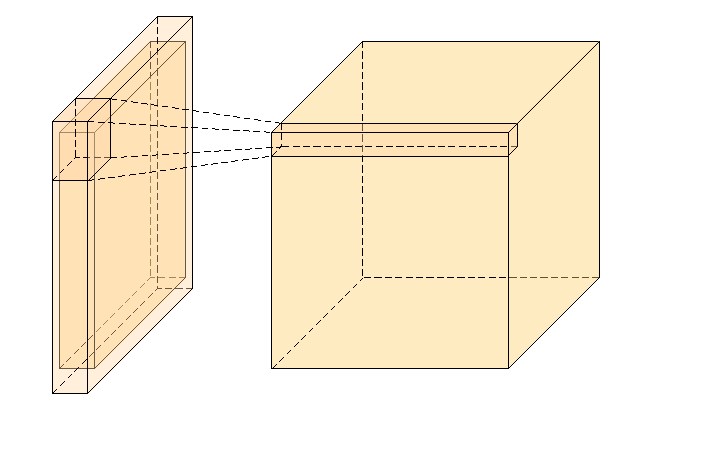
\includegraphics[width=\textwidth]{images/convolution.pdf}
         \caption{}
         \centering
     \end{subfigure}
     \hfill
     \caption{Illustration of how a convolution layer works. The input layer is shown on the left, where each pixel has a number of values associated with it (e.g.~RGB values for a standard image). In order to calculate values for the next layer, only values contained within a square surrounding each pixel are summed together. The depth of the right hand block represents the number of channels evaluated over each pixel. On the input image, the padding is shown as the lighter shaded box surrounding the smaller box. See text for further discussion of this figure. }
     \label{fig:conv_nn}
\end{figure}




There are many ways of connecting nodes in a layer to those in the next layer; the layers shown in this example, where every node is connected to all nodes in the next layer, are known as \emph{dense} layers. For applications involving images, an effective choice of connectivity between layers is to use \emph{convolutions}, resulting in a \emph{convolutional neural network} (CNN)~\citep{oshea_introduction_2015}. A diagram illustrating how a layer in a CNN works is shown in Fig.~\ref{fig:conv_nn}: Connectivity between layers is limited so that only pixels within a square surrounding the pixel in question are summed over. We may apply many convolutions each with different weightings to sum around the same pixel; these different weightings are called \emph{channels}, and they are represented in Fig.~\ref{fig:conv_nn} in the extended depth of the block on the right hand side. Note that for pixels at the edges we cannot apply a convolution, which makes the output smaller than the input, which may not be desirable. To avoid this, extra values can be inserted around the edges of the input (`padding'), so that a convolution can also be applied at the edges (represented as the lighter larger box on the left hand side in Fig.~\ref{fig:conv_nn}). There are many different choices of padding, such as padding with zeros, and `reflect' padding where the padding is the reflection of the values near the edge. 

Another key building block of neural networks used in this work is a \emph{residual block}~\citep{he_deep_2016}. The idea behind the residual block is that, to avoid over-fitting (whereby the model is too highly tuned to the training data), we may want to allow the network to leave out any blocks of neurons that do not help the model generalise. A residual block passes the input $\mathbf{x}$ through two layers (convolutional layers with padding in our case), and then adds the input to the output $\mathbf{y}$ of these layers. In situations where this block is not useful for improving the model performance, the model can then learn to bypass these operations more easily. 

A vital property of artificial neural networks is the ability to efficiently update the parameters based on errors in the outputs, via the backpropagation algorithm. In this algorithm, a suitable loss function is chosen that quantifies the errors between the model output and the target values (e.g.~mean square error). Then these errors can be propagated backwards to calculate what changes to the neural network parameters will improve the performance. Training then proceeds by many of these updates using a suitable optimisation algorithm.

A key consideration when training a machine learning model is how to partition the data to produce a model that performs optimally. To achieve this, data is often split into three partitions; the training set (which is typically much larger than the other two partitions), the validation set, and the test set. To begin with, the model is trained on the training data and evaluated on the (unseen) validation data, using a variety of parameters and architecture choices, in order to get a sense of what the best model setup is for the data. Once the best performing model has been chosen based on the validation set, it is evaluated on the test set and these results reported. This enables the model to be tuned whilst reducing the chance of tuning the model to the particular test set. When partitioning our data like this, we ideally want all three datasets to be drawn from the same distribution. One way of ensuring this would be to ignore the time-ordering of the data so that all three datasets are sampled over the same time period; however, this is problematic because samples in the training set can be correlated with those in the validation and test set, so the performance of the model on the validation and test set is not a true reflection of the model performance on unseen data. Additionally, in an operational setting it is common to have a model trained on historical data that then acts on current data. Therefore, with data that varies in time, it is common to order the datasets so that the training precedes the validation set, which precedes the test set. We provide details of the particular train/validation/test split used in this work in Sec.~\ref{sec:model_setup}


\section{Machine learning for numerical weather prediction}

Much of the work incorporating cutting edge machine learning techniques into numerical weather prediction has occurred relatively recently, using techniques that are well established in the machine learning community. Most if not all of the state-of-the art models use artificial neural networks. In~\cite{chantry_opportunities_2021} they split the use of machine learning for weather prediction into three different categories `Hard', `Medium' and `Soft' AI.

Using this categorisation, Hard AI refers to training a forecasting model based purely on large amounts of observational or reanalysis data. There have been particularly high profile attempts at doing this, such as using a Generative Adversarial Network to nowcast precipitation~\citep{ravuri_skilful_2021}, graph neural networks for short to medium range global forecasting of many variables~\citep{lam_graphcast_2022}, nowcasting models that learn via an advection scheme~\citep{zhang_skilful_2023}, and using transformers for nowcasting and short-range forecasts of many variables~\citep{nguyen_climax_2023, bi_pangu-weather_2022}. Generative models are particularly relevant for weather prediction as they can generate arbitrary numbers of forecasts, and so provide a method to create an ensemble, which is typically more useful as it allows a quantification of risks~\citep{palmer_economic_2002}. 

% refs in Nguyne et al.: Weyn Durran et al 2020
% Keisler graph neural network

These fundamental models have shown impressive results, and have the potential to provide forecasts at higher speeds and resolutions than can be achieved using physical models. However, there is still uncertainty about how reliable and robust they are compared to existing physical models, since most implementations are not trained to obey conservation laws (although there have been several works demonstrating how some conservation laws can be incorporated into neural network training~\citep{beucler_enforcing_2019, harder_generating_2022}). This is especially important for predicting extremes, or for making projections of a future climate where past observations may not allow us to predict the weather under novel conditions. Additionally, there are technical limitations, in that the these models require huge amounts of high-quality data that may not be available. 

Machine learning models are also trained to align with particular observations or reanalysis data, and so it is often hard to rigorously compare them to physical models that aren't designed to align with the same data (especially given the lack of a forecast verification metric that aligns with human intuitions of forecast quality). Additionally, where models are trained on reanalysis data, there is an implicit dependence on physical models, and no guarantee that they also perform well against other observation datasets~\citep{ramavajjala_verification_2023}.

For these reasons, in the short term at least, there are advantages to pursue a Medium AI approach, where a machine learning model adjusts the outputs of the physical model based on observations, or where it replaces a particular component of the physical model (such as a parameterization schemes). As argued in~\cite{watson_applying_2019}, this approach could be advantageous in that the core forecast comes from a model that obeys the laws of physics, whilst the corrections applied by the machine learning model are typically smaller and so any deviations from physical realism should be less significant. It also means that behaviours that are captured well by the physical models can still be used and do not need to be re-learnt by the model. 

Several works have demonstrated the ability of artificial neural networks to improve the spatial variability and correct intensity biases of forecasts for fields such as precipitation and temperature~\citep{rasp_neural_2018, steininger_convmos_2022, duncan_generative_2022}. Additionally, these models have been shown to perform well at increasing the resolution of precipitation forecasts (`downscaling'), both using using deterministic models~\citep{sha_deep-learning-based_2020, wang_deep_2021, vandal_intercomparison_2019, rampal_high-resolution_2022, mishra_sharma_resdeepd_2022} and generative models~\citep{harris_generative_2022, leinonen_stochastic_2020}. 

Finally, in the Soft AI approach, machine learning models act as emulators of components in a physical model, or as part of the assimilation process. The usefulness of machine learning in this case is not in improving forecast skill, but in increasing the efficiency of forecasting systems. For example,~\cite{krasnopolsky_using_2013} and~\cite{brenowitz_prognostic_2018} use a neural network to emulate the behaviour of a high resolution cloud-resolving model, to represent the overall effect of this model at a coarser grid scale.



% In many cases, such as tropical rainfall forecasting that we deal with here, the forecast model may not have been developed to work optimally in the particular area of interest, and so it makes sense to have some sort of postprocessing.

% The performance of a model is also multi-faceted, and different forecast users may be more interested in having forecasts that perform well at different tasks; for example one user may only require that the forecasts perform well at the grid cell without concern for spatial realism, whilst others 

% there are many downstream users of a forecast who are concerned with different aspects of a forecast, then the ability to easily post-process to better match a particular set of observations may be advantageous.
 

% Whilst these fundamental models have shown impressive results, there is still uncertainty about how reliable and robust they are compared to existing physics-based models, especially at the extremes or in regimes such as climate change where past observations may not allow us to predict the weather under novel conditions. It is also hard to know what conclusions to draw from these models because:

% \begin{itemize}
% \item Models are typically trained on root mean square error, which is known to be problematic for fields like precipitation because of the double-penalty problem~\citep{wilks_forecast_2019}.
% \item They have not yet been subjected to the same level of scrutiny that established operational models have. 
% \item Existing forecasts aren't designed to align with a particular observation or reanalysis data, unlike a model that is trained to do so.
% \item Existing models are often trained on reanalysis products like ERA5 which require a physical model to produce, and may contain information about the future.
% \item Whilst models may align well with reanalysis, that gives no guarantee they also perform well against observations~\citep{ramavajjala_verification_2023}.
% \end{itemize}




% % See~\citep{Vannitsem2021StatisticalWorld}. Additionally 



% ........
% Summary of hybrid approaches to e.g.~hydroclimate prediction (includes seasonal and medium range forecasts of precipitation) discussed in~\citep{slater_hybrid_2023}. One advantage; when there are many downstream use-cases of a forecasting product,


% Fine if we're only forecasting one variable, but if we want many the speed / cost / accuracy benefits are not as clear.

% AI could be good alternatives to limited area model; cheaper to produce ensemble members and so better for multivariate considerations.

\ifSubfilesClassLoaded{%
    \bibliographystyle{alpha}
    \bibliography{references_z}

}{}


\end{document}